\chapter{Introduction}
\label{Introduction}

\section{Freshwater degradation on large scales}
\label{Freshwater degradation on large scales}

The current epoch of Anthropocene has been marked by an extensive degradation of world's ecosystems by a multitude of natural, and particularly, anthropogenic stressors (Crutzen, 2006). Freshwater ecosystems are among the most extensively degraded and hence, are threatened by a considerable loss of biodiversity and a substantial reduction of secured freshwater supply for human consumptions (Carpenter et al., 2011; Dudgeon et al., 2005; Millennium Ecosystem Assessment (MEA), 2005; Vörösmarty et al., 2010). The planetary boundary for biodiversity loss has already been exceeded (Rockström et al., 2009; Steffen et al., 2015); the populations of more than 300 freshwater species have declined up to 55\% during 1970-2000 (UNEP, 2015; WWF, 2015). Moreover, 23\% of the world's largest streams have experienced a significant decrease in flow and discharge during 1948 – 2004 (Dai et al., 2009). If the current trend prevails, a 15 – 37\% loss of freshwater biodiversity and a substantial decrease of discharge in 40\% of the world's largest streams are anticipated by 2050 (Stocker et al., 2013; UNEP, 2015; WWF, 2015). Moreover, two-third of world's population, especially inhabitants of developing countries, are predicted to be in moderate to severe water stress by 2025 (MEA, 2005; Vörösmarty et al., 2010). Overall, freshwater degradation may entail unprecedented and irreversible human and ecological impacts in the coming decades.

Degradation of freshwater resources has mainly been triggered by four groups of stressors: (i) catchment land use, e.g. overexploitation of water resources, (ii) water pollution, e.g. excessive nutrients and toxicants, (iii) water resources development, e.g. flow modification and river morphological changes, and (iv) biotic factors, e.g. invasive species (Dudgeon et al., 2005; Vörösmarty et al., 2010).  Climate change, which is a large scale environmental stressor and adversely affects freshwater ecosystems through an increase in the frequency of extreme events such as droughts and floods as well as by changing temperature regimes and discharge patterns (Dai et al., 2009; Stocker et al., 2013; Vörösmarty, 2000), superimposes upon these four groups of stressors (Dudgeon et al., 2005). Different global regions have been evidencing single and joint effects of these stressors on their freshwater resources, while many stressors exhibited spatial concordance in their magnitude (Table 1.1) (Vörösmarty et al., 2010). Moreover, there is an increasing risk of exceeding planetary boundaries for land use and climate change, and the boundary for freshwater use has already been exceeded in arid and semi-arid regions (Steffen et al., 2015). Consequently, availability of suitable habitats for freshwater species have been shrinking and many species, which cannot adapt or emigrate, have been extinct (Pereira et al., 2010; IUCN, 2015; Walther et al., 2002). Human migrations have also been evidenced due to freshwater degradation, especially from developing countries with constrained mitigation capabilities, leading to freshwater stress in receiving areas (McLeman and Smit, 2006; Reuveny, 2007).

\begin{table}[h]
\label{Table 1.1}
\caption{Degradation of freshwater resources in different regions of the world by a single and confounding effects of natural and anthropogenic stressors.}
\begin{threeparttable}
\centering
\begin{tabular}{>{\centering\arraybackslash}m{1.8cm}>{\centering\arraybackslash}m{2.0cm}>{\centering\arraybackslash}m{2.0cm}>{\centering\arraybackslash}m{3.5cm}>{\centering\arraybackslash}m{2.5cm}}

\toprule
\textbf{Spatial scale} & \textbf{Region} & \textbf{Potentially affected freshwater bodies} & \textbf{Major stressors and stressor groups
} & \textbf{Source}\\

\midrule

Global & World & 68 \% & Agricultural insecticides & Stehle and Schulz, (2015) \\
\hline
\multirow{3}{*}{Continental} & \multirow{2}{*}{Europe} & 50 \% & Water pollution, water resources development and catchment land use & EEA (2012)\\
\cline{3-5}
 & & 42 \% & Organic chemicals & Malaj et al. (2014)\\
 \cline{2-5}
 & Asia & 67 \% & Water pollution and catchment land use & UNEP (2008)\\
 \hline
\multirow{4}{*}{Nationwide} & United States of America & 53 \% & Water pollution and water resources development & USEPA (2015)\\
\cline{2-5}
 & Australia & 55 \% & Salinity, nutrients and sediments & Lovett et al. (2007); NLWRA (2002)\\
\cline{2-5}
 & Germany & 80 \% & Water pollution, water resources development and catchment land use & Dahm et al. (2013); EEA (2012)\\
 \cline{2-5}
 & China & 60 \% & Water pollution & MEPA China (2009)\\

\bottomrule

\end{tabular}
\begin{tablenotes}
\footnotesize
Note: the assessments are based on different metrics (see the sources)
\end{tablenotes}
\end{threeparttable}
\end{table}

In response to extensive freshwater degradation, and with the aim of preserving existing freshwater bodies with good qualities and restoring good qualities of degraded waterbodies, several political frameworks have been developed, e.g. European Water Framework Directive (EC, 2010) and the Blueprint to Safeguard Europe’s Water Resources (EC, 2013). These frameworks, based on the classical view that ecological communities are strongly influenced by species interactions within local habitats, exclusively focus on small scale approaches, e.g. stream reach scales, and rarely account for large scale degradations (EC, 2013, 2010; Hugueny et al., 2010). Biomonitoring related to these frameworks directly monitor biological quality elements (BQE), i.e. organism groups such as fish, benthic invertebrates, macrophytes and diatoms, which reflect freshwater degradation in general, in stream reaches to identify locally degraded habitats for restoration (EC, 2013, 2010). However, local and regional species richness often exhibit positive relationships and thus indicate that local communities are also affected by large scale drivers, such as climate, which in turns entail alternations in community patterns on large scales (Hugueny et al., 2010). Hence, large scale assessments of stressors effects are important for enabling integrated management of freshwater resources. Moreover, large scale approaches may complement local scale stream restoration by indicating potentially degraded areas for prioritization (Heino et al., 2013; Hugueny et al., 2010). Large scale managements, such as catchment based managements, also support a transboundary preservation and restoration of freshwater resources because streams and lakes often flow across national borders (EC, 2010).

While the existing frameworks are working with strict deadlines to achieve targeted freshwater quality in the developed part of the world, developing countries under severe freshwater stress are still lacking for such initiatives due to resource constraints and sparse information on stressors (EC, 2010; MEPA China, 2014; UNEP, 2008). For many developing countries, regional scale assessments of freshwater degradation are unavailable and total human and freshwater species populations at risk are still unknown. Thus, the implementation of freshwater management frameworks in water-stressed developing countries inherently depends on the large scale assessments of human and ecological impacts of freshwater degradation by filling data gaps. Novel methods accounting for data scarcity are thus required that can also combine large scale secondary databases and used them to predict freshwater degradation (Hengl, 2009). Moreover, large scale approaches may help to optimize the usage of limited resources, i.e. resource mobilization and expansion of water quality monitoring to potentially degraded areas predicted by large scale approaches (Törnqvist et al., 2011).

\newpage

\section{Spatial models for freshwater ecological analyses}
\label{Spatial models for freshwater ecological analyses}

Spatial models, ensembles of geographical information systems (GIS)\textsuperscript{\textbf{1}} and spatiotemporal statistics (hereafter spatial statistics (SS)\textsuperscript{\textbf{2}}), have become essential tools in freshwater research, especially for large scale analyses (Fortin and Dale, 2005; Legendre and Legendre, 1998). Non-random distribution of freshwater entities and freshwater ecosystem processes over space and time lead to spatial and temporal dimensions in freshwater ecological phenomena (Legendre and Fortin, 1989). Spatiotemporal patterns resulting from freshwater ecological processes are often exogenous, i.e. spatiotemporally driven by numerous natural and anthropogenic processes. However, they may also be endogenous, i.e. causally related to ecological interactions, and inherent biological and physiological processes (Legendre and Legendre, 1998).

\bigskip

\noindent\fcolorbox{white}{Gray}{

\begin{minipage}{\textwidth}

\begin{description}

\item[1. Geographical information systems (GIS)] --- Geographical information systems (GIS) are computer-coupled systems that enable digital storage, processing and retrieval of georeferenced (with coordinate information of locations on the earth surface) data, and visualization of outputs in a map (Vogiatzakis, 2003). Mapping earthly phenomena has been a major human activity since the first civilizations. However, the first GIS was developed and implemented by Canadian Cartographic Association in 1975 for the preparation of a digital cartographic database of the country (CCA, 2015). The concept of GIS was first formalized by Parent and Church (1987), who outlined it as a decision making tool using geographic data, i.e. data on natural landscapes. Later in 1989, GIS were shown to be an efficient decision making tool for everything happening over space (earth surface), i.e. natural and anthropogenic processes, and thus were established as systems of rather spatial data than geographic data (Anselin, 1989). Time as a dimension started receiving equal importance as space and hence, was integrated with GIS, which transformed the concept of GIS into “spatiotemporal information systems” (Burrough and Frank, 1995). The rapid evolution of GIS and its extensive application across disciplines highlighted the role of science behind it and eventually conceived “geographical information science” as a new field and an integrated part of the available GIS (Goodchild, 1992).

Spatial (angular or projected coordinates) and temporal (time step, interval or series) attributes are stored in GIS along with the data attributes, e.g. species richness and trace metal concentration, and are explicitly used for data analyses (Chrisman, 2001). The analyses are performed to answer spatiotemporal location and scale-based questions, e.g. where and when is the species richness high or low? What is the scale of pollution from trace metals? Maps of different data layers can be overlaid and used to answer questions regarding interactions between spatiotemporal phenomena, e.g. is species richness low at the location with and time of high trace metal concentration? Different data layers can also be merged to compute multi-metric indices, e.g. locations or years with both high trace metal concentration and high deforestation are at higher ecological risk than the locations with only high trace metal concentration or high deforestation (Burrough and Frank, 1995).

Integration of GIS with ecological modelling entailed considerable development in ecological resource inventory and analyses, and exhibited substantial improvement in decision making for ecological management (Vogiatzakis, 2003). Parallel developments in the fields using spatiotemporal data, i.e. photogrammetry and remote sensing, result in substantial advancement in GIS including the development of multiple platforms and algorithms that enable processing of large scale ecological datasets (Fortin and Dale, 2005; Legendre and Legendre, 1998).

\end{description}

\end{minipage}}

\bigskip

Large-scale drivers, such as climate and land use, are often spatially autocorrelated\textsuperscript{\textbf{2}}. Moreover, transport and propagation of pollutants, such as agricultural insecticides and industrial metals, are spatially related to the terrain characteristics as well as to the physicochemical characteristics of soil and water and sources of anthropogenic pollution (Huang et al., 2015; Winkel et al., 2008). Spatial autocorrelation of these natural and anthropogenic drivers induce spatial patterns in the distribution of freshwater species and human settlements (Legendre, 1993). Thus, particularly understanding exogenous patterns in freshwater ecological processes and their causes are the key to disentangle stressors effects on large scales. Spatial models or the spatially explicit ecological models help to understand the exogenous spatial patterns by incorporating spatial dimensions (spatial locations) into ecological models\textsuperscript{\textbf{1,2}}.

\bigskip

\noindent\fcolorbox{white}{Gray}{

\begin{minipage}{\textwidth}

\begin{description}

\item[2. Spatial statistics (SS)] --- Spatial statistics (SS) is the field of statistics that involves quantitative analyses of data with spatial attributes (i.e. coordinates) and modelling of their spatial variability and uncertainty (Chiles and Delfiner, 2012). The inherent assumption of SS is spatial autocorrelation, which is derived from Tobler’s first law of geography – “everything is related to everything else, but near things are more related than distant things” (Tobler, 1970). Natural and anthropogenic processes on the earth surface at pairs of locations, which are a certain distance apart tend to be more similar (positive spatial autocorrelation) or dissimilar (negative spatial autocorrelation) than at randomly associated pairs of locations (Legendre, 1993). Thus, spatial autocorrelation, typically measured with Moran's I and Geary's C, computes the degree to which a set of spatial observations tend to be clustered together or dispersed on space (Fortin and Dale, 2005). SS is used for the analyses of patterns and uncertainty of data exhibiting spatial autocorrelation by including the distance decay in the similarity or dissimilarity of attribute values.

SS includes: (i) geostatistics, i.e. spatial prediction of continuous and random processes, and variability at unsampled locations, (ii) areal statistics, i.e. pattern and variability analyses for areal (non-point), gridded (regularly spaced) and remotely sensed data, and (iii) point pattern statistics, i.e. pattern analyses in randomly and sparsely distributed point data (Gaetan et al., 2010). Geostatistics have been extensively applied in the variability analyses of spatially continuous natural and anthropogenic processes, e.g. climate and pollution (Christakos, 2000). Spatial variability analysis is typically conducted by ``variograms'', where variances (semivariances) between attribute values of certain point pairs are plotted against their separation distances (lags). Patterns of variabilities identified by the models fitted to variograms are employed through spatial interpolation techniques, e.g. kriging, for spatial prediction of attribute values at non-sampled locations (Webster and Oliver, 2007). Spatial regression models, e.g. geographically weighted regression, are applied for spatial prediction with areal data, such as regional level water pollution (Harris et al., 2010). Biogeography of species and exposures from toxicants are typically identified by point pattern statistics, which includes identification of spatial clusters, trends and density (Cressie, 1993).

\end{description}

\end{minipage}}

\bigskip

Spatial dimensions of ecological processes have always been an implicit part of the freshwater ecological framework (Legendre, 1993). However, models incorporating spatial attributes and autocorrelation have only recently been explicitly integrated in freshwater ecological sampling, experiment and analyses, especially on large scales (Fortin et al., 2012). Ecological datasets are generally multivariate and location specific (Vogiatzakis, 2003). The complexity of large scale ecological problems demands combination of large datasets from diverse sources and of different level of details (resolutions) with ecological datasets (Vogiatzakis, 2003). In fact, analyses of large scale human and ecological impacts of stressors, i.e. quantification of stressors on catchment and regional scales, assessment of large scale entity-driver relationships and risk assessments, require answers to several spatial questions\textsuperscript{\textbf{1}} in ecological phenomena and understanding of the interactions between ecological entities and drivers across spatial scales (Borcard et al., 2004). GIS facilitates the combination of large datasets of different sources and resolutions with ecological datasets as well as their joint and efficient processing for disentangling spatial heterogeneity and ecological interactions across spatial scales (Vogiatzakis, 2003). SS enable quantitative analyses of stressors, entity-driver relationships and large scale risks within GIS in the context of earth change (Gaetan et al., 2010). Hence, the integration of spatial models with ecological models fosters large scale human and ecological impact assessments from freshwater degradation.

The integration of spatial models with ecological models can be done in two ways (see Figure 1.1 for details): (i) running ecological models separately, and use spatial models for pre-processing, e.g. coordinate transformation and reprojection, and post processing of the data, e.g. mapping and overlaying, and (ii) running spatial and ecological models interactively on the same platform so that they can share databases with common data structures and perform ecological analyses inside GIS using SS (Vogiatzakis, 2003). The former integration entails problems due to lack of common data models, structures and interface, whereas the latter entails advantages due to the capability of including spatial operators, e.g. distance, and spatial propagation of errors into the model. Multiple platforms have been developed facilitating the interactive integration of spatial models with ecological models for spatially enabled ecological analyses (ESRI, Redlands, 2001; GRASS Development Team, 2015; R Development Core Team, 2015). These platforms enable co-interfacing of spatial and ecological models for performing GIS and SS analyses on large ecological datasets for answering spatial-ecological questions (Figure 1.1).

\section{Catchment and regional scale stressors quantification}
\label{Catchment and regional scale stressors quantification}

Ecological status and health of freshwater resources, and potential disturbance at biological endpoints, e.g. community of stream invertebrates, are typically monitored at reach-scale and stream sampling points (SSP) (Biss et al., 2006; Stevens Jr and Olsen, 2004). Stressors occurring on catchment scales, such as climate change and pollution, may exhibit causal relationships with the ecological status and communities observed at these outlet stream reaches and SSPs (Dahm et al., 2013; Lorenz and Feld, 2013; Marzin et al., 2013). Moreover, environmental quality at catchments often represent the quality of outlet stream reaches (Skøien et al., 2014). Hence, large scale analyses to complement small scale management often require quantification of the extent and variability of stressors on catchments and in turns require catchment delineation for stream reaches and SSPs.

GIS, through the development in the field of remote sensing, have made high resolution digital elevation models (DEM)\textsuperscript{\textbf{3}} readily available that enables efficient delineation of stream catchments for stream reaches and SSPs  (Abood et al., 2012; Fernández et al., 2012; Holmes and Goebel, 2011; Lagacherie et al., 2010). However, this requires extraction of a stream network from DEMs by tracing water flow generated by terrain characteristics, that accurately approximates the actual stream network on earth surface (Ver Hoef et al., 2014). Although stream extraction from DEMs exhibited considerable advancement over field survey and traditional digitization techniques, and extraction steps have largely been automated, the most crucial step, i.e. selection of an accumulation threshold (AT) (see chapter 2 for a more detailed description) that distinguishes between stream and non-stream cells, is still done arbitrarily (Tarboton et al., 1991). This leads to laborious and manual (visual) comparison of DEM extracted stream networks with traditionally mapped stream network. A few automated AT selection algorithms were developed on proprietary software and only tested for small scale datasets (Heine et al., 2004; Lin et al., 2006). Hence, they are not accessible and jeopardize large scale stream extractions from DEMs. Furthermore, stressors such as land use, pollution and flow modification often act at at the upstream reach scale, i.e. upstream riparian corridors (URC), and affect stream communities at outlet SSPs (Dahm et al., 2013). Therefore, studies investigating stressor impacts on stream communities often require delineation of the URCs for given SSPs (Lorenz and Feld, 2013). However, no algorithm has been developed to perform automated delineation of URCs for given SSPs and sizes to date, and hence they are often manually drawn (Colson et al., 2008). To conclude, freely accessible and automated algorithms are required for objective selection of ATs and efficient delineation of URCs for given SSPs.

Regional scale drivers, such as climate, exhibit spatial continuity and hence, regional gridded surfaces representing their variability and magnitude are essential for identification of stress from their dynamics as well as to predict stress at locations, where indices representing these drivers were

\begin{landscape}
\noindent\begin{figure}[t]
  \centering
  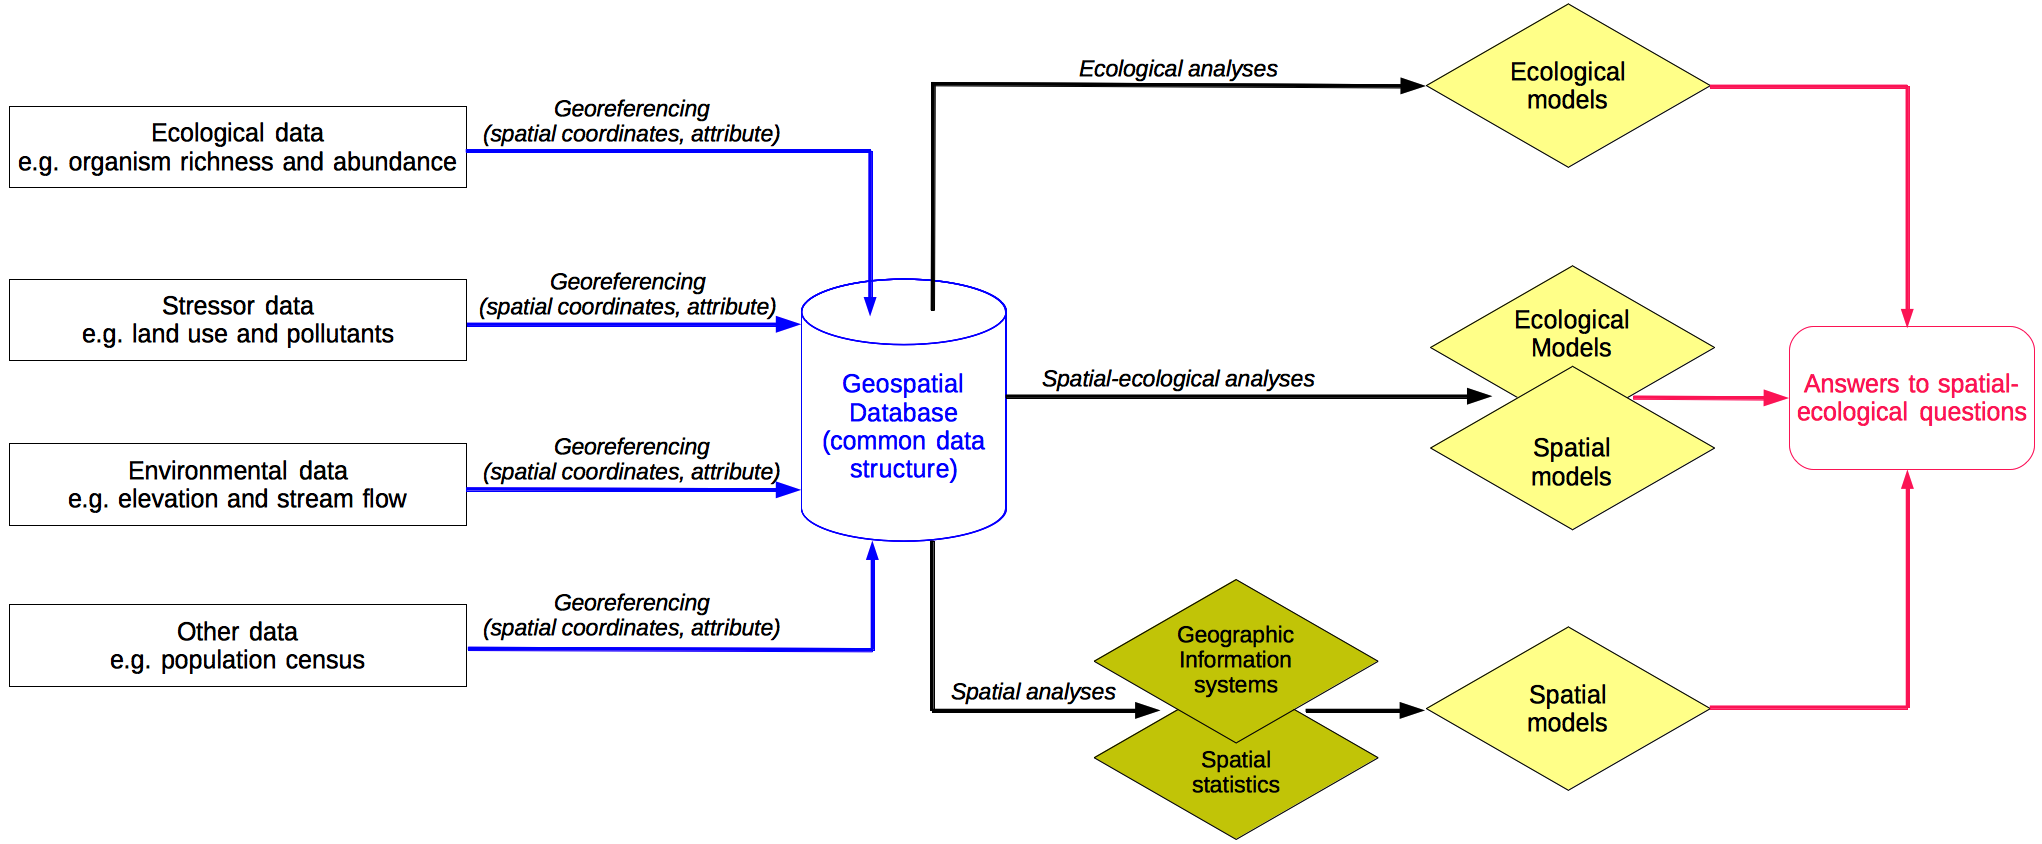
\includegraphics[width=\linewidth]{Figures/Fig_1_1.png}
  \caption{Integration of spatial models with ecological models for spatial-ecological analyses (adopted from the description in Vogiatzakis (2003)).}
  \label{Fig_1_1}
\end{figure}

\noindent not sampled (Webster and Oliver, 2007). Geostatistical interpolation techniques, e.g. kriging\textsuperscript{\textbf{2}}, have been extensively applied for the prediction of variability and magnitude of these indices at non-sampled locations (Hengl, 2009). Spatial variograms\textsuperscript{\textbf{2}}, which model spatial variability of indices, play a central role in geostatistical interpolation, and the number and density of observations in a region are crucial for precise variogram estimation (Webster and Oliver, 2007). In developing countries, observations are often scarce and sparsely distributed because of constrained resources that lead to an unsatisfactory precision of variogram estimation (Goovaerts, 1997; Parajka et al., 2015). Pooled variogram estimation (see chapter 3 for details), which is conducted by comparing spatial variability from multiple time steps, e.g. years, in the presence of time series data, delivers a considerable increase in precision of variogram estimation

\end{landscape}

\noindent\fcolorbox{white}{Gray}{

\begin{minipage}{\textwidth}

\begin{description}

\item[3. Digital elevation model (DEM)] --- A digital elevation model (DEM) is a digital model of the earth surface created from terrain elevation (height from the mean sea level) data (Li et al., 2004). Generally, they are represented as rasters (collection of square grids), where each raster cell represents a location on the earth surface and contains height information of that location. The size of the cell is called resolution and represents the level of details of information in a DEM. However, DEMs can also be represented by a vector-based triangular irregular network (TIN). DEMs are also interchangeably used as digital terrain model (DTM) and digital surface model (DSM) (Hengl, 2009). Nevertheless, DEMs only contain elevation information of the earth, whereas, DTMs, in addition, contain information on the shape of the earth and containing objects, and DSMs contain bare earth shape information. DEMs are generally created using remote sensing techniques, i.e. based on the imageries taken by interferometric synthetic aperture radars boarded on airplanes or earth observation satellites, e.g. ASTER (NASA and METI, 2009; Wise, 2007). They provide important information on earth surface pattern and terrain characteristics that are frequently used in many research fields, e.g. hydrology, cartography and geography (Saunders, 2000).

\end{description}

\end{minipage}}

\bigskip

\noindent under data scarcity (Schuurmans et al., 2007; Wagner et al., 2012). However, the available method for pooled variogram estimation averages variograms estimated for individual time steps that are not suitable for time series with varying spatial locations and number of data points (typical case for developing countries) (Goovaerts, 1997; Gräler et al., 2011). Hence, to increase the precision of pooled variogram estimation, an alternative method is required that account for the variable number and locations of data points in a time series.

\section{Large scale spatial relationship between biological quality elements and drivers}
\label{Large scale spatial relationship between biological quality elements and drivers}

Freshwater organism groups have frequently been used as biological quality elements (BQE) for computation of indices, which are used to indicate the ecological status of freshwater bodies (EC, 2010; Kenney et al., 2009). Especially, traits\textsuperscript{\textbf{4}} of organism groups have shown considerable potential as indicators of multiple stressor effects in freshwater ecosystems (Kenney et al., 2009; Statzner and Bêche, 2010; Van den Brink et al., 2011). They have exhibited substantially less variation than taxonomic groups and hence, demonstrate particularly high suitability for large scale assessment of freshwater degradation and stressor effects (Bonada et al., 2007). Traits have successfully indicated pollution from toxic sediments (Archaimbault et al., 2009), alteration in catchment land use (Larsen and Ormerod, 2010), climate change (Lawrence et al., 2010), salinity and habitat degradation (Díaz et al., 2007), nutrient loads (Dolédec et al., 2006), organic contamination and hydrological disturbances (Feio and Dolédec, 2012) across spatial scales. They also demonstrated high predictive potential for recovery of organisms from degradation (Shipley et al., 2006) and were shown to provide links to important ecosystem functions and services (Mlambo, 2014; Vandewalle et al., 2010).

Many studies have used \textit{a priori} traits of freshwater organisms as biotic indicators of degradation and to disentangle effects of multiple stressors. For example, trait-based approaches have been applied to identify ecological risk from cooccurrences of stressors (Davies and Jackson, 2006), pesticides (Liess et al., 2008), salinity (Kefford et al., 2006) and organic toxicants (Beketov and Liess, 2008; Ohe et al., 2009). Moreover, traits that were hypothesized to be vulnerable to climate change were used to identify organism groups and stream sites that may potentially be at the highest risk of the adverse effects of climate change (Conti et al., 2013; Sandin et al., 2014). However, the spatial relationship between organismal traits and these drivers have rarely been examined on large scales. This limits our macroecological knowledge of the potential spatial responses of organismal traits to large scale drivers, which is important for understanding the change in large scale distribution patterns of freshwater communities under stress (Dray et al., 2012; Heino et al., 2013).

\bigskip

\noindent\fcolorbox{white}{Gray}{

\begin{minipage}{\textwidth}

\begin{description}

\item[4. Traits] --- Traits are biological (phenotypic) and ecological attributes that corresponds to individual and average states of organisms (Van den Brink et al., 2011). These attributes evolve from a number of developmental, morphological, physiological and behavioral adaptations of organisms to their environment (Lancaster and Downes, 2010a, 2010b). Biological traits refer to the life history characteristics, e.g. body size, life cycle, feeding habits and reproduction, whereas ecological traits refer to the ecological preferences of organisms, e.g. habitat, current and temperature preferences (Vandewalle et al., 2010). Traits represent functional characteristics of organisms and thus promote mechanistic understanding of biological communities in a taxon independent manner (Mlambo, 2014; Vandewalle et al., 2010). Hence, trait information can be compared across ecosystems and used to establish links between community and ecosystem ecology (Schmera et al., 2015). A typical trait database contains the affinity (score) of organisms or organism groups to certain traits that are grouped under representative features, e.g. body sizes of $<$ 0.25 cm and 0.25 - 0.50 cm are grouped under the body size featuring group. The largest trait database for European freshwater species is “Freshwater Ecology” (\href{http://www.freshwaterecology.info/}{http://www.freshwaterecology.info/}).

\end{description}

\end{minipage}}

\section{Large scale human and ecological risk assessment}
\label{Large scale human and ecological risk assessment}

Large scale human and ecological risk assessments from stressors, such as contaminants are essential for identification of potential hot spots to develop management strategies and reduce anthropogenic inputs (EEA, 2012). Moreover, the total population at risk from multiple stressors need to be identified for remediation of contaminated areas (Srinivasa and Govil, 2007). However, due to the unavailability of large scale (nationwide, continental and global) contaminant monitoring data, large scale risk assessment are often impeded (Malaj et al., 2014). For example, planetary boundary for global chemical contamination could not be determined although effects on ecosystem health have been evidenced on a global scale (Rockström et al., 2009; Steffen et al., 2015). Especially, in developing countries, resource constraints often limit water quality monitoring activities to a few locations and hence, nationwide risk assessments are often not available and information on the extent of stress and the total population at risk is largely unknown (Azizullah et al., 2011; Törnqvist et al., 2011). Moreover, the monitoring is often biased against rural and remote areas, where people having the least access to water purification measures may be affected by the degradation at upstream urban areas (Khan et al., 2008). Lack of nationwide risk assessments, in turn, impede development of freshwater management frameworks in water-stressed developing countries (MEPA China, 2014; UNEP, 2008). To this end, large scale assessments of human and ecological risks from contaminants are important for the formation of new frameworks in developing countries. While development of large scale contaminant monitoring datasets, e.g. the European Waterbase Dataset (EEA, 2012), are resource and time intensive and in many cases impossible for developing countries, spatial prediction techniques can be employed to fill data gaps for non-sampled locations and enable large scale risk assessments (Javi et al., 2014; Nas and Berktay, 2010).

\section{Aims and objectives}
\label{Aims and objectives}

This Ph.D. thesis aims at: (i) developing novel spatial tools and methods for catchment and regional scale quantification of stressors, (ii) examining large scale relationships between freshwater assemblage traits and drivers by integrating spatial models with ecological models, and (iii) assessing nationwide human health risks from contaminants in data scarce developing countries. Four studies have been conducted using large scale datasets covering three global regions (Figure 1.2), which are presented in chapters 2 – 5 (see Figure 1.3 for the workflow of this thesis).

In chapter 2, an automated and open-source tool is outlined for accumulation threshold (AT) selection that enables objective stream network extraction and upstream riparian corridor (URC) delineation for given stream sampling points from digital elevation models. The objectives of this study were:

\begin{itemize}
\item to develop an algorithm for an automatic and objective selection of ATs by ensuring the highest concordance between DEM extracted and traditionally mapped stream networks
\item to develop an algorithm for automatic and accurate delineation of URCs for given SSPs and sizes, by snapping SSPs to DEM extracted and approximated stream networks
\item to validate and test these algorithms for large scale datasets
\end{itemize}

Chapter 3 outlines an alternative method for pooled within-time series variogram estimation for scarce hydrological data by spatially shifting temporal data points. Specific objectives were:

\begin{itemize}
\item to develop an alternative method for pooled variogram estimation that account for variable numbers and location of data points in a time series
\item to compare the precision of variogram estimation of the developed method with the available method in a data scarce region
\end{itemize}

Large scale relationships between aquatic insect assemblage traits and climate are described in chapter 4, which were established using biomonitoring data from 4,752 German stream sites and 35 global bioclimatic indices (BIs). Spatial variability and autocorrelation in the distribution of aquatic insects were quantified and checked for their association with the BIs. The objectives of this study were:

\begin{itemize}
\item to identify traits and insect groups showing the strongest spatial relationship with the global BIs
\item to identify traits and insect groups showing the highest potential for changing distribution under future climate change
\end{itemize}

\vspace{-0.5cm}\noindent\begin{figure}[h!]
  \centering
  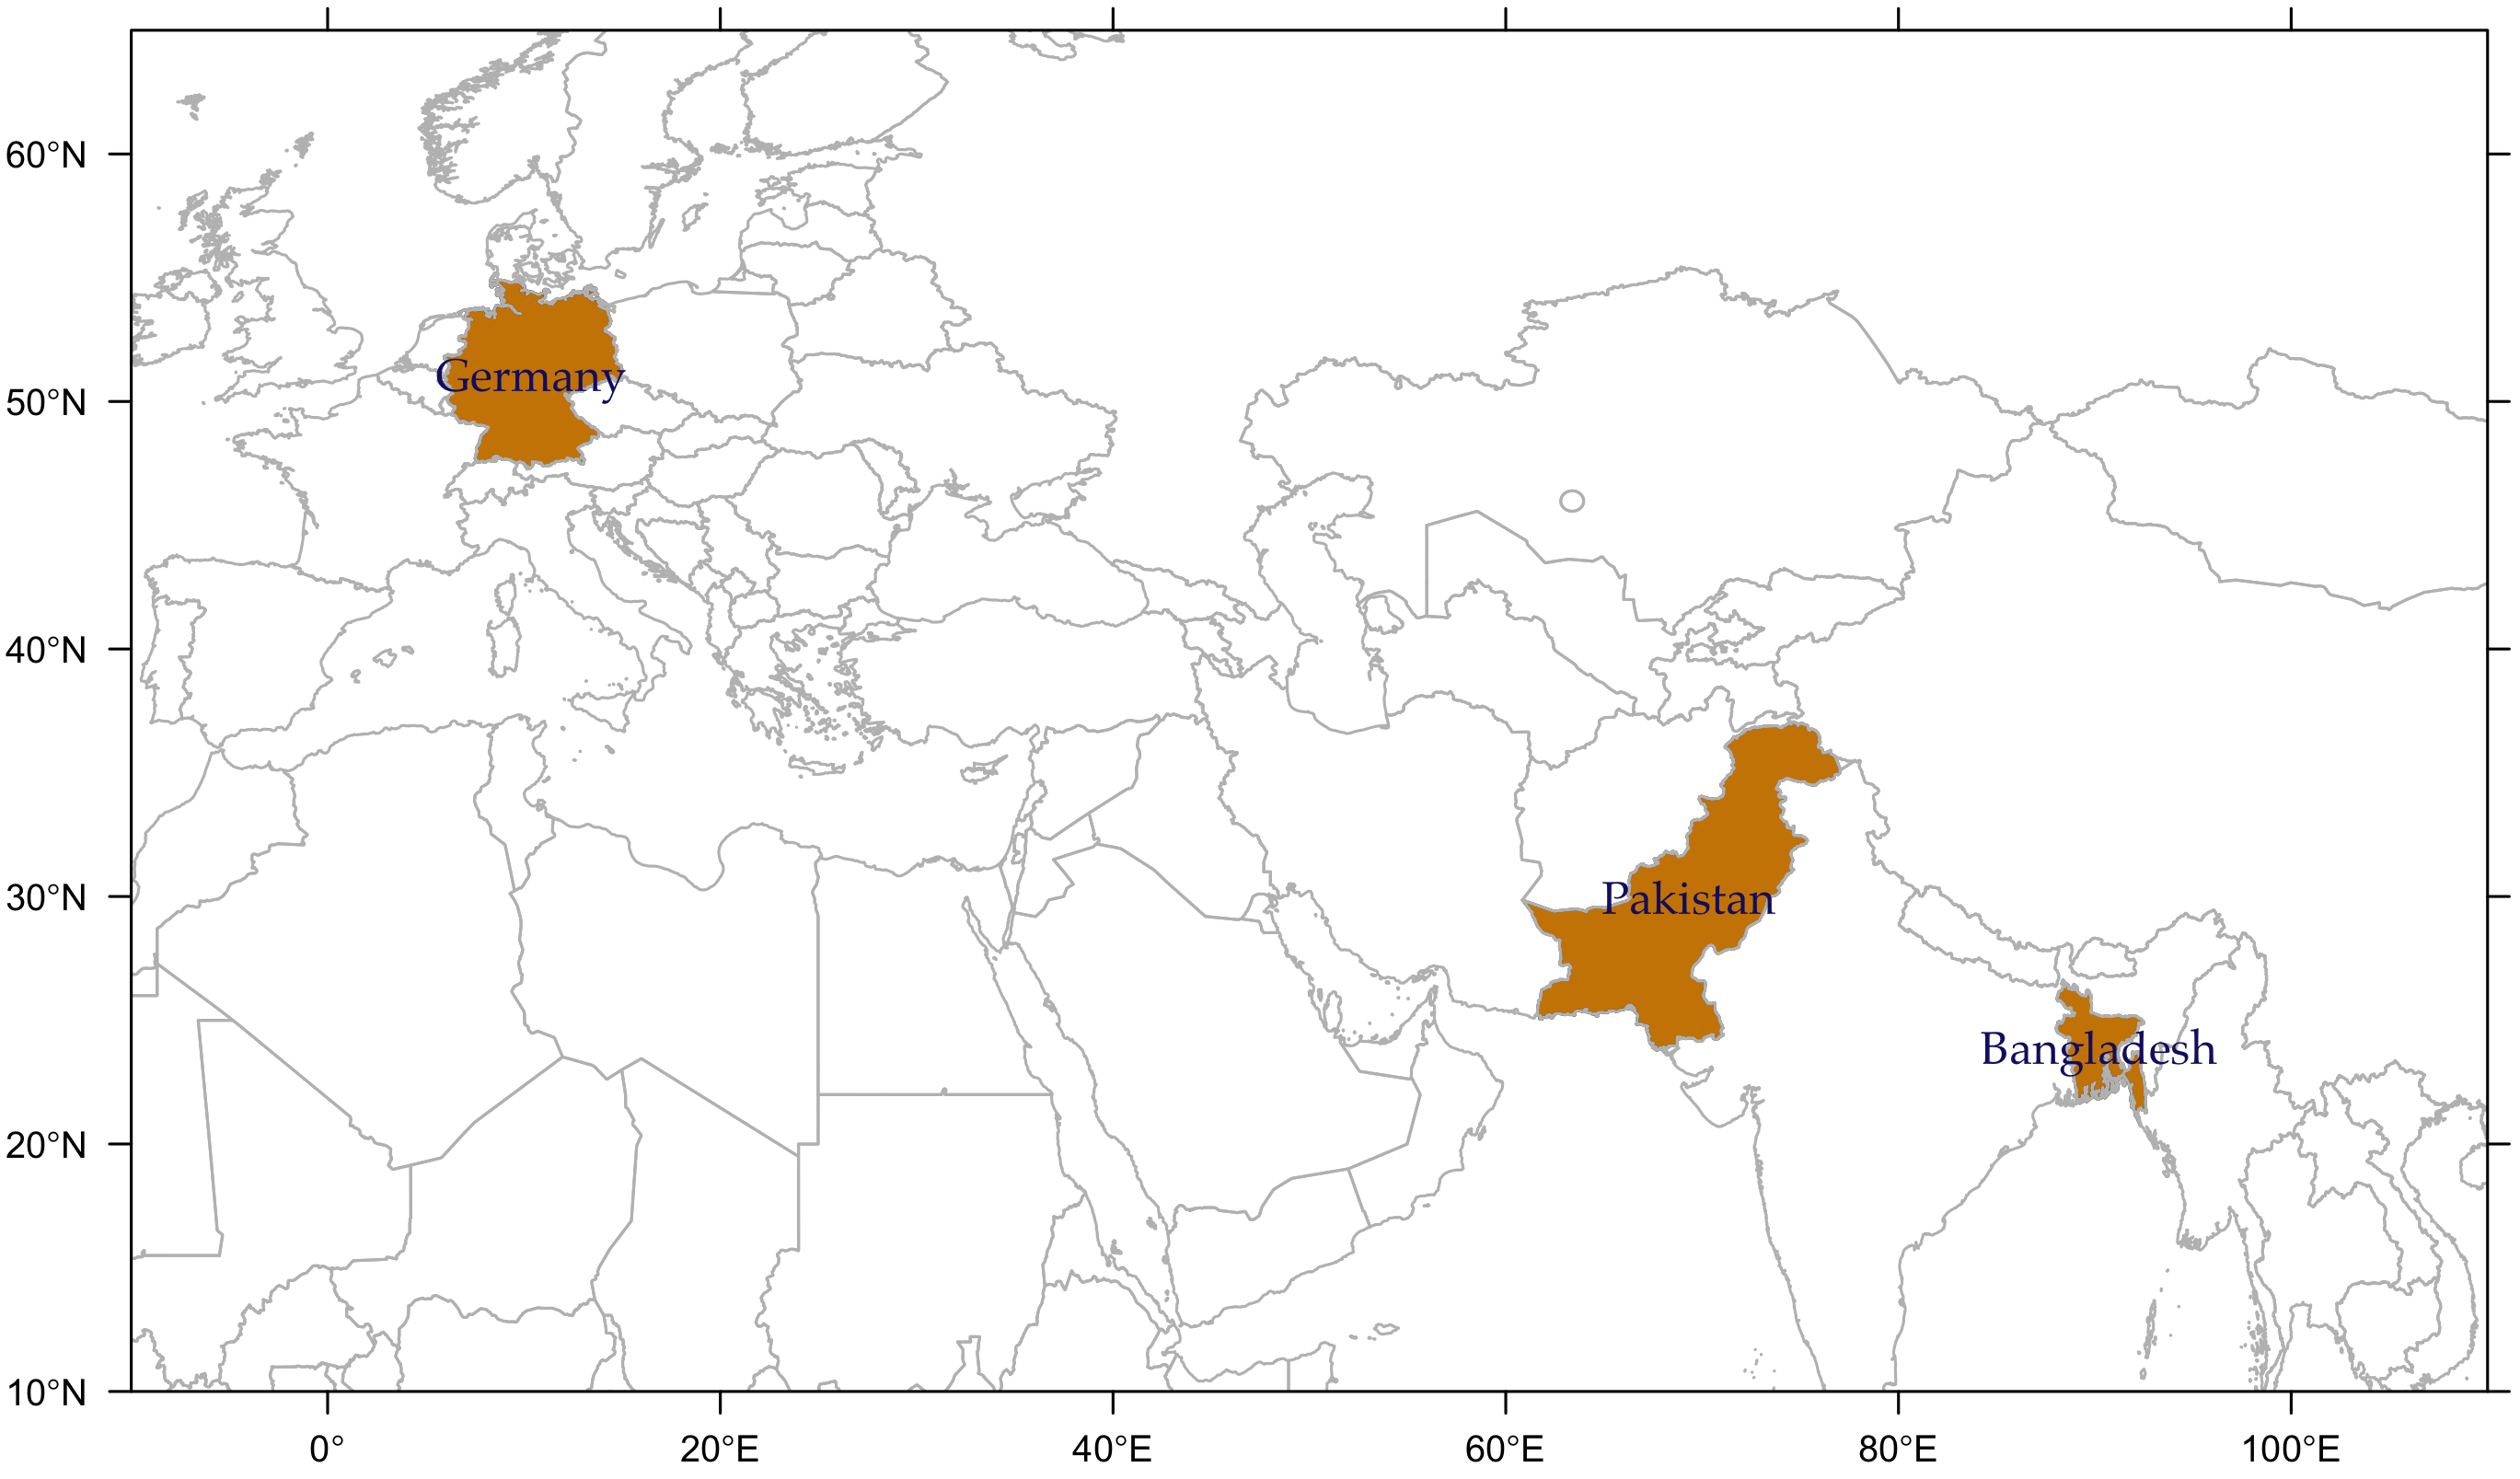
\includegraphics[width=\linewidth]{Figures/Fig_1_2.png}
  \caption{Three global regions (highlighted in orange) covered by the studies in this thesis.}
  \label{Fig_1_2}
\end{figure}

\clearpage

\noindent\begin{figure}[h!]
  \centering
  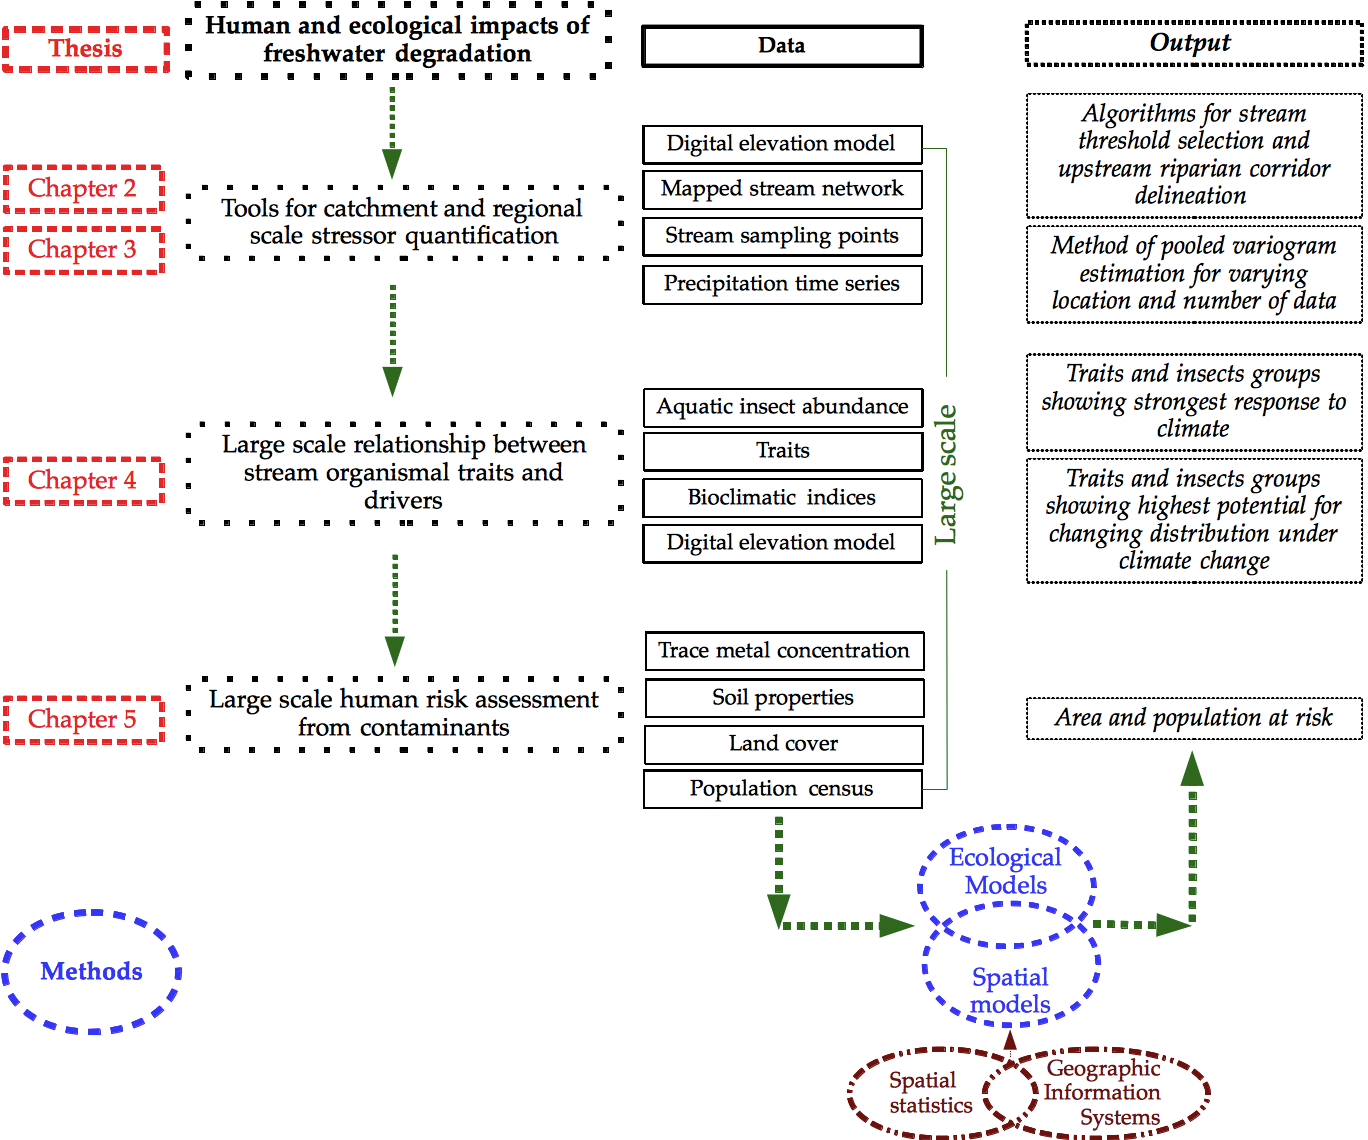
\includegraphics[width=\linewidth]{Figures/Fig_1_3.png}
  \caption{Schematic diagram of the work-flow of this thesis}
  \label{Fig_1_3}
\end{figure}

Finally, a large scale human health risk assessment is described in chapter 5 from trace metal contamination of drinking water sources in Pakistan. A spatial prediction technique that accounts for data scarcity and thus large distances between samples was employed with several spatial predictors for large scale prediction of trace metal concentrations in ground and surface water. The predicted concentrations were compared to the guideline values for drinking water to assess human health risk and quantify total area and population at risk. The objectives were:

\begin{itemize}
\item to predict the concentrations of 10 trace metal in ground and surface water by employing an appropriate spatial prediction technique on previously published data for a few administrative area and using relevant spatial predictors
\item to use predicted trace metal concentrations for nationwide human health risk assessment by comparing with guideline values and quantify total area and population at risk.
\end{itemize}

\begingroup

\renewcommand{\addcontentsline}[3]{}

\begin{thebibliography}

\bibitem{} \hangindent=1cm Abood, S.A., Maclean, A.L., Mason, L.A., 2012. Modeling Riparian Zones Utilizing DEMS and Flood Height Data. Photogrammetric engineering and remote sensing 78, 259–269.

\bibitem{} \hangindent=1cm Anselin, L., 1989. What is special about spatial data?: alternative perspectives on spatial data analysis. Presented at the Spatial Statistics, Past, Present and Future, Syracuse.

\bibitem{} \hangindent=1cm Archaimbault, V., Usseglio-Polatera, P., Garric, J., Wasson, J.-G., Babut, M., 2009. Assessing pollution of toxic sediment in streams using bio-ecological traits of benthic macroinvertebrates: Toxic pollution index and macroinvertebrates. Freshwater Biology 55, 1430–1446. doi:10.1111/j.1365-2427.2009.02281.x

\bibitem{} \hangindent=1cm Azizullah, A., Khattak, M.N.K., Richter, P., Häder, D.-P., 2011. Water pollution in Pakistan and its impact on public health — A review. Environment International 37, 479–497. doi:10.1016/j.envint.2010.10.007

\bibitem{} \hangindent=1cm Beketov, M.A., Liess, M., 2008. An indicator for effects of organic toxicants on lotic invertebrate communities: Independence of confounding environmental factors over an extensive river continuum. Environmental Pollution 156, 980–987. doi:10.1016/j.envpol.2008.05.005

\bibitem{} \hangindent=1cm Biss, R., Kübler, P., Pinter, I., Braukmann, U., 2006. Leitbildbezogenes biozönotisches Bewertungsverfahren für Fließgewässer in der Bundesrepublik Deutschland -Ein erster Beitrag zur integrierten ökologischen Fließgewässerbewertung (Project report No. 298 24 777), UBA-FB 000348. Umweltforschungsplan des Bundesministeriums für Umwelt, Naturschutz und Reaktorsicherheit, Berlin.

\bibitem{} \hangindent=1cm Bonada, N., DoléDec, S., Statzner, B., 2007. Taxonomic and biological trait differences of stream macroinvertebrate communities between mediterranean and temperate regions: implications for future climatic scenarios. Global Change Biology 13, 1658–1671. doi:10.1111/j.1365-2486.2007.01375.x

\bibitem{} \hangindent=1cm Borcard, D., Legendre, P., Avois-Jacquet, C., Tuomisto, H., 2004. Dissecting the spatial structure of ecological data at multiple scales. Ecology 85, 1826–1832.

\bibitem{} \hangindent=1cm Burrough, P.A., Frank, A.U., 1995. Concepts and paradigms in spatial information: are current geographical information systems truly generic? International journal of geographical information systems 9, 101–116. doi:10.1080/02693799508902028

\bibitem{} \hangindent=1cm Canadian Cartographic Association (CCA), 2015. Canadian Cartographic Association [WWW Document]. URL http://cca-acc.org/about-us/ (accessed 8.14.15).

\bibitem{} \hangindent=1cm Carpenter, S.R., Stanley, E.H., Vander Zanden, M.J., 2011. State of the World’s Freshwater Ecosystems: Physical, Chemical, and Biological Changes. Annual Review of Environment and Resources 36, 75–99. doi:10.1146/annurev-environ-021810-094524

\bibitem{} \hangindent=1cm Chiles, J.-P., Delfiner, P., 2012. Geostatistics modeling spatial uncertainty, second edition. John Wiley & Sons, Hoboken, N.J.
Chrisman, N., 2001. Exploring geographical information systems. Wiley.

\bibitem{} \hangindent=1cm Christakos, G., 2000. Modern spatiotemporal geostatistics. Courier Corporation.

\bibitem{} \hangindent=1cm Colson, T., Gregory, J., Dorney, J., Russell, P., 2008. Topographic and soil maps do not accurately depict headwater stream networks. National Wetlands Newsletter 30, 25–28.

\bibitem{} \hangindent=1cm Conti, L., Schmidt-Kloiber, A., Grenouillet, G., Graf, W., 2013. A trait-based approach to assess the vulnerability of European aquatic insects to climate change. Hydrobiologia 721, 297–315. doi:10.1007/s10750-013-1690-7

\bibitem{} \hangindent=1cm Cressie, N., 1993. Statistics for spatial data, Revised edition. ed. John Wiley & Sons, New York, Chichester, Toronto, Brisbane, Singapore.

\bibitem{} \hangindent=1cm Crutzen, P., 2006. The “Anthropocene,” in: Ehlers, E., Krafft, T. (Eds.), Earth System Science in the Anthropocene. Springer Berlin Heidelberg, pp. 13–18.

\bibitem{} \hangindent=1cm Dahm, V., Hering, D., Nemitz, D., Graf, W., Schmidt-Kloiber, A., Leitner, P., Melcher, A., Feld, C.K., 2013. Effects of physico-chemistry, land use and hydromorphology on three riverine organism groups: a comparative analysis with monitoring data from Germany and Austria. Hydrobiologia 704, 389–415. doi:10.1007/s10750-012-1431-3

\bibitem{} \hangindent=1cm Dai, A., Qian, T., Trenberth, K.E., Milliman, J.D., 2009. Changes in continental freshwater discharge from 1948 to 2004. Journal of Climate 22, 2773–2792.

\bibitem{} \hangindent=1cm Davies, S.P., Jackson, S.K., 2006. The biological condition gradient: a descriptive model for interpreting change in aquatic ecosystems. Ecological Applications 16, 1251–1266.

\bibitem{} \hangindent=1cm DíAz, A.M., Alonso, M.L.S., GutiéRrez, M.R.V.-A., 2007. Biological traits of stream macroinvertebrates from a semi-arid catchment: patterns along complex environmental gradients. Freshwater Biology 0, 071204011451001–??? doi:10.1111/j.1365-2427.2007.01854.x

\bibitem{} \hangindent=1cm Dolédec, S., Phillips, N., Scarsbrook, M., Riley, R.H., Townsend, C.R., 2006. Comparison of structural and functional approaches to determining landuse effects on grassland stream invertebrate communities. Journal of the North American Benthological Society 25, 44–60. doi:10.1899/0887-3593(2006)25[44:COSAFA]2.0.CO;2

\bibitem{} \hangindent=1cm Dray, S., Pélissier, R., Couteron, P., Fortin, M.-J., Legendre, P., Peres-Neto, P.R., Bellier, E., Bivand, R., Blanchet, F.G., De Cáceres, M., 2012. Community ecology in the age of multivariate multiscale spatial analysis. Ecological Monographs 82, 257–275. doi:10.1890/11-1183.1

\bibitem{} \hangindent=1cm Dudgeon, D., Arthington, A.H., Gessner, M.O., Kawabata, Z.-I., Knowler, D.J., Lévêque, C., Naiman, R.J., Prieur-Richard, A.-H., Soto, D., Stiassny, M.L.J., Sullivan, C.A., 2005. Freshwater biodiversity: importance, threats, status and conservation challenges. Biological Reviews 81, 163–182. doi:10.1017/S1464793105006950

\bibitem{} \hangindent=1cm Environmental Systems Research Institute (ESRI), Redlands, 2001. What is ArcGIS?: GIS by ESRI. ESRI.

\bibitem{} \hangindent=1cm European Commission (EC), 2013. A blueprint to safeguard Europe’s water resources, NAT.

\bibitem{} \hangindent=1cm European Commission (EC), 2010. Water Framework Directive.

\bibitem{} \hangindent=1cm European Environment Agency (EEA), 2012. European waters - assessment of status and pressures (No. 8/2012). European Environment Agency, Copenhagen.

\bibitem{} \hangindent=1cm Feio, M.J., Dolédec, S., 2012. Integration of invertebrate traits into predictive models for indirect assessment of stream functional integrity: a case study in Portugal. Ecological Indicators 15, 236–247.

\bibitem{} \hangindent=1cm Fernández, D., Barquín, J., Álvarez-Cabria, M., Peñas, F.J., 2012. Quantifying the performance of automated GIS-based geomorphological approaches for riparian zone delineation using digital elevation models. Hydrology and Earth System Sciences 16, 3851–3862. doi:10.5194/hess-16-3851-2012

\bibitem{} \hangindent=1cm Fortin, M.-J., Dale, M.R.T., 2005. Spatial analysis: a guide for ecologists. Cambridge University Press, Cambridge.

\bibitem{} \hangindent=1cm Fortin, M.-J., James, P.M.A., MacKenzie, A., Melles, S.J., Rayfield, B., 2012. Spatial statistics, spatial regression, and graph theory in ecology. Spatial Statistics 1, 100–109. doi:10.1016/j.spasta.2012.02.004

\bibitem{} \hangindent=1cm Gaetan, C., Guyon, X., Bleakley, K., 2010. Spatial statistics and modeling. Springer.

\bibitem{} \hangindent=1cm Goodchild, M.F., 1992. Geographical information science. International journal of geographical information systems 6, 31–45.

\bibitem{} \hangindent=1cm Goovaerts, P., 1997. Geostatistics for natural resources evaluation. Oxford university press.

\bibitem{} \hangindent=1cm Gräler, B., Gerharz, L.E., Pebesma, E., 2011. Spatio-temporal analysis and interpolation of PM10 measurements in Europe (Technical paper No. 2011/10). European Topic Center on Air Pollution and Climate Change Mitigation, Bilthoven.

\bibitem{} \hangindent=1cm GRASS Development Team, 2015. Geographic Resources Analysis Support System (GRASS). Open Source Geospatial Foundation Project.

\bibitem{} \hangindent=1cm Harris, P., Fotheringham, A.S., Crespo, R., Charlton, M., 2010. The Use of Geographically Weighted Regression for Spatial Prediction: An Evaluation of Models Using Simulated Data Sets. Mathematical Geosciences 42, 657–680. doi:10.1007/s11004-010-9284-7

\bibitem{} \hangindent=1cm Heine, R.A., Lant, C.L., Sengupta, R.R., 2004. Development and Comparison of Approaches for Automated Mapping of Stream Channel Networks. Annals of the Association of American Geographers 94, 477–490. doi:10.1111/j.1467-8306.2004.00409.x

\bibitem{} \hangindent=1cm Heino, J., Schmera, D., Erős, T., 2013. A macroecological perspective of trait patterns in stream communities. Freshwater Biology 58, 1539–1555. doi:10.1111/fwb.12164

\bibitem{} \hangindent=1cm Hengl, T., 2009. A Practical Guide to Geostatistical Mapping. University of Amsterdam, Amsterdam.

\bibitem{} \hangindent=1cm Holmes, K.L., Goebel, P.C., 2011. A functional approach to riparian area delineation using geospatial methods. Journal of Forestry 109, 233–241.

\bibitem{} \hangindent=1cm Huang, J., Huang, Y., Pontius, R.G., Zhang, Z., 2015. Geographically weighted regression to measure spatial variations in correlations between water pollution versus land use in a coastal watershed. Ocean & Coastal Management 103, 14–24. doi:10.1016/j.ocecoaman.2014.10.007

\bibitem{} \hangindent=1cm Hugueny, B., Oberdorff, T., Tedesco, P.A., 2010. Community ecology of river fishes: a large-scale perspective, in: American Fisheries Society Symposium. pp. 29–62.

\bibitem{} \hangindent=1cm International Union for Conservation of Nature (IUCN), 2015. International Union for Conservation of Nature [WWW Document]. URL http://www.iucn.org/ (accessed 8.13.15).

\bibitem{} \hangindent=1cm Javi, S.T., Malekmohammadi, B., Mokhtari, H., 2014. Application of geographically weighted regression model to analysis of spatiotemporal varying relationships between groundwater quantity and land use changes (case study: Khanmirza Plain, Iran). Environmental Monitoring and Assessment 186, 3123–3138. doi:10.1007/s10661-013-3605-5

\bibitem{} \hangindent=1cm Kefford, B.J., Nugegoda, D., Metzeling, L., Fields, E.J., 2006. Validating species sensitivity distributions using salinity tolerance of riverine macroinvertebrates in the southern Murray-Darling Basin (Victoria, Australia). Canadian Journal of Fisheries and Aquatic Sciences 63, 1865–1877.

\bibitem{} \hangindent=1cm Kenney, M.A., Sutton-Grier, A.E., Smith, R.F., Gresens, S.E., 2009. Benthic macroinvertebrates as indicators of water quality: The intersection of science and policy. Terrestrial Arthropod Reviews 2, 99–128. doi:10.1163/187498209X12525675906077

\bibitem{} \hangindent=1cm Khan, S., Cao, Q., Zheng, Y.M., Huang, Y.Z., Zhu, Y.G., 2008. Health risks of heavy metals in contaminated soils and food crops irrigated with wastewater in Beijing, China. Environmental Pollution 152, 686–692. doi:10.1016/j.envpol.2007.06.056

\bibitem{} \hangindent=1cm Lagacherie, P., Rabotin, M., Colin, F., Moussa, R., Voltz, M., 2010. Geo-MHYDAS: A landscape discretization tool for distributed hydrological modeling of cultivated areas. Computers & Geosciences 36, 1021–1032. doi:10.1016/j.cageo.2009.12.005

\bibitem{} \hangindent=1cm Lancaster, J., Downes, B.J., 2010a. Linking the hydraulic world of individual organisms to ecological processes: Putting ecology into ecohydraulics. River Research and Applications 26, 385–403. doi:10.1002/rra.1274

\bibitem{} \hangindent=1cm Lancaster, J., Downes, B.J., 2010b. Ecohydraulics needs to embrace ecology and sound science, and to avoid mathematical artefacts. River Research and Applications 26, 921–929. doi:10.1002/rra.1425

\bibitem{} \hangindent=1cm Larsen, S., Ormerod, S.J., 2010. Combined effects of habitat modification on trait composition and species nestedness in river invertebrates. Biological Conservation 143, 2638–2646. doi:10.1016/j.biocon.2010.07.006

\bibitem{} \hangindent=1cm Lawrence, J.E., Lunde, K.B., Mazor, R.D., Bêche, L.A., McElravy, E.P., Resh, V.H., 2010. Long-term macroinvertebrate responses to climate change: implications for biological assessment in mediterranean-climate streams. Journal of the North American Benthological Society 29, 1424–1440. doi:10.1899/09-178.1

\bibitem{} \hangindent=1cm Legendre, P., 1993. Spatial Autocorrelation: Trouble or New Paradigm? Ecology 74, 1659. doi:10.2307/1939924

\bibitem{} \hangindent=1cm Legendre, P., Fortin, M.J., 1989. Spatial pattern and ecological analysis. Vegetatio 80, 107–138.

\bibitem{} \hangindent=1cm Legendre, P., Legendre, L.F., 1998. Numerical ecology. Elsevier.

\bibitem{} \hangindent=1cm Liess, M., Schäfer, R.B., Schriever, C.A., 2008. The footprint of pesticide stress in communities—Species traits reveal community effects of toxicants. Science of The Total Environment 406, 484–490. doi:10.1016/j.scitotenv.2008.05.054

\bibitem{} \hangindent=1cm Lin, W.T., Chou, W.C., Lin, C.Y., Huang, P.H., Tsai, J.S., 2006. Automated suitable drainage network extraction from digital elevation models in Taiwan’s upstream watersheds. Hydrological Processes 20, 289–306. doi:10.1002/hyp.5911

\bibitem{} \hangindent=1cm Li, Z., Zhu, C., Gold, C., 2004. Digital terrain modeling: principles and methodology. CRC press.

\bibitem{} \hangindent=1cm Lorenz, A.W., Feld, C.K., 2013. Upstream river morphology and riparian land use overrule local restoration effects on ecological status assessment. Hydrobiologia 704, 489–501. doi:10.1007/s10750-012-1326-3

\bibitem{} \hangindent=1cm Lovett, S., Price, P., Edgar, B., 2007. Salt, nutrient, sediment and interactions: findings from the National River contaminants program. Land and Water Australia, Canberra, A.C.T.

\bibitem{} \hangindent=1cm Malaj, E., Peter, C., Grote, M., Kühne, R., Mondy, C.P., Usseglio-Polatera, P., Brack, W., Schäfer, R.B., 2014. Organic chemicals jeopardize the health of freshwater ecosystems on the continental scale. Proceedings of the National Academy of Sciences 201321082.

\bibitem{} \hangindent=1cm Marzin, A., Verdonschot, P.F.M., Pont, D., 2013. The relative influence of catchment, riparian corridor, and reach-scale anthropogenic pressures on fish and macroinvertebrate assemblages in French rivers. Hydrobiologia 704, 375–388. doi:10.1007/s10750-012-1254-2

\bibitem{} \hangindent=1cm McLeman, R., Smit, B., 2006. Migration as an Adaptation to Climate Change. Climatic Change 76, 31–53. doi:10.1007/s10584-005-9000-7

\bibitem{} \hangindent=1cm Millennium Ecosystem Assessment (MEA), 2005. Ecosystems and human well-being: wetlands and water (Synthesis). World Resources Institute, Washington, D.C.

\bibitem{} \hangindent=1cm Ministry of Environmental Protection, the People’s Republic of China (MEPA China), 2014. The State of the Environment of China in 2013 [WWW Document]. URL http://english.mep.gov.cn/ (accessed 8.13.15).

\bibitem{} \hangindent=1cm Mlambo, M.C., 2014. Not all traits are “functional”: insights from taxonomy and biodiversity-ecosystem functioning research. Biodiversity and Conservation 23, 781–790. doi:10.1007/s10531-014-0618-5

\bibitem{} \hangindent=1cm Nas, B., Berktay, A., 2010. Groundwater quality mapping in urban groundwater using GIS. Environmental Monitoring and Assessment 160, 215–227. doi:10.1007/s10661-008-0689-4

\bibitem{} \hangindent=1cm National Aeronautics and Space Administration (NASA), Japan’s Ministry of Economy, Trade and Industry (METI), 2009. ASTER Global Digital Elevation Map [WWW Document]. URL http://asterweb.jpl.nasa.gov/gdem.asp (accessed 12.18.13).

\bibitem{} \hangindent=1cm National Land & Water Resources Audit, Australia (NLWRA), 2002. Australian catchment, river, and estuary assessment 2002: assessing the aggregate impact of resource use on key natural ecosystems. (No. ISBN: 0 642 37125 3). National Land & Water Resources Audit, Canberra ACT.

\bibitem{} \hangindent=1cm Ohe, P.C. von der, De Deckere, E., Prü\s s, A., Muñoz, I., Wolfram, G., Villagrasa, M., Ginebreda, A., Hein, M., Brack, W., 2009. Toward an integrated assessment of the ecological and chemical status of European river basins. Integrated environmental assessment and management 5, 50–61.

\bibitem{} \hangindent=1cm Parajka, J., Merz, R., Skøien, J.O., Viglione, A., 2015. The role of station density for predicting daily runoff by top-kriging interpolation in Austria 63. doi:10.1515/johh-2015-0024

\bibitem{} \hangindent=1cm Parent, P., Church, R., 1987. Evolution of Geographic Information Systems as Decision Making Tools, in: Proceedings of the 2nd Annual Conference on Geographic Information Systems. Presented at the 2nd Annual Conference on Geographic Information Systems, San Francisco, pp. 63–71.

\bibitem{} \hangindent=1cm Pereira, H.M., Leadley, P.W., Proenca, V., Alkemade, R., Scharlemann, J.P.W., Fernandez-Manjarres, J.F., Araujo, M.B., Balvanera, P., Biggs, R., Cheung, W.W.L., Chini, L., Cooper, H.D., Gilman, E.L., Guenette, S., Hurtt, G.C., Huntington, H.P., Mace, G.M., Oberdorff, T., Revenga, C., Rodrigues, P., Scholes, R.J., Sumaila, U.R., Walpole, M., 2010. Scenarios for Global Biodiversity in the 21st Century. Science 330, 1496–1501. doi:10.1126/science.1196624

\bibitem{} \hangindent=1cm Pollard, A.I., Yuan, L., 2006. Community response patterns: evaluating benthic invertebrate composition in metal-polluted streams. Ecological Applications 16, 645–655.

\bibitem{} \hangindent=1cm R Development Core Team, 2015. R: A language and environment for statistical computing. R Foundation for Statistical Computing. Vienna, Austria.

\bibitem{} \hangindent=1cm Reuveny, R., 2007. Climate change-induced migration and violent conflict. Political Geography 26, 656–673. doi:10.1016/j.polgeo.2007.05.001

\bibitem{} \hangindent=1cm Rockström, J., Steffen, W.L., Noone, K., Persson, \AAsa, Chapin III, F.S., Lambin, E., Lenton, T.M., Scheffer, M., Folke, C., Schellnhuber, H.J., others, 2009. Planetary boundaries: exploring the safe operating space for humanity.

\bibitem{} \hangindent=1cm Sandin, L., Schmidt-Kloiber, A., Svenning, J.-C., Jeppesen, E., Friberg, N., 2014. A trait-based approach to assess climate change sensitivity of freshwater invertebrates across Swedish ecoregions. Current Zoology 60.

\bibitem{} \hangindent=1cm Saunders, W., 2000. Preparation of DEMs for use in environmental modeling analysis. Hydrologic and hydraulic modeling support with geographic information systems. ESRI Press, New York 29–52.

\bibitem{} \hangindent=1cm Schmera, D., Podani, J., Heino, J., Erős, T., Poff, N.L., 2015. A proposed unified terminology of species traits in stream ecology. Freshwater Science 000–000. doi:10.1086/681623

\bibitem{} \hangindent=1cm Schuurmans, J.M., Bierkens, M.F.P., Pebesma, E.J., Uijlenhoet, R., 2007. Automatic Prediction of High-Resolution Daily Rainfall Fields for Multiple Extents: The Potential of Operational Radar. Journal of Hydrometeorology 8, 1204–1224. doi:10.1175/2007JHM792.1

\bibitem{} \hangindent=1cm Shipley, B., Vile, D., Garnier, E., 2006. From Plant Traits to Plant Communities: A Statistical Mechanistic Approach to Biodiversity. Science 314, 812–814. doi:10.1126/science.1131344

\bibitem{} \hangindent=1cm Skøien, J.O., Blöschl, G., Laaha, G., Pebesma, E., Parajka, J., Viglione, A., 2014. rtop: an R package for interpolation of data with a variable spatial support, with an example from river networks. Computers & Geosciences. doi:10.1016/j.cageo.2014.02.009

\bibitem{} \hangindent=1cm Srinivasa, S.G., Govil, P.K., 2007. Distribution of heavy metals in surface water of Ranipet industrial area in Tamil Nadu, India. Environmental Monitoring and Assessment 136, 197–207. doi:10.1007/s10661-007-9675-5

\bibitem{} \hangindent=1cm Statzner, B., Bêche, L.A., 2010. Can biological invertebrate traits resolve effects of multiple stressors on running water ecosystems? Freshwater Biology 55, 80–119. doi:10.1111/j.1365-2427.2009.02369.x

\bibitem{} \hangindent=1cm Steffen, W., Richardson, K., Rockstrom, J., Cornell, S.E., Fetzer, I., Bennett, E.M., Biggs, R., Carpenter, S.R., de Vries, W., de Wit, C.A., Folke, C., Gerten, D., Heinke, J., Mace, G.M., Persson, L.M., Ramanathan, V., Reyers, B., Sorlin, S., 2015. Planetary boundaries: Guiding human development on a changing planet. Science 347, 1259855–1259855. doi:10.1126/science.1259855

\bibitem{} \hangindent=1cm Stehle, S., Schulz, R., 2015. Agricultural insecticides threaten surface waters at the global scale. Proceedings of the National Academy of Sciences 112, 5750–5755. doi:10.1073/pnas.1500232112

\bibitem{} \hangindent=1cm Stevens Jr, D.L., Olsen, A.R., 2004. Spatially balanced sampling of natural resources. Journal of the American Statistical Association 99, 262–278.

\bibitem{} \hangindent=1cm Stocker, T.F., Dahe, Q., Plattner, G.-K., 2013. Climate Change 2013: The Physical Science Basis, Working Group I Contribution to the Fifth Assessment Report of the Intergovernmental Panel on Climate Change. Summary for Policymakers. Intergovernmental Panel on Climate Change (IPCC).

\bibitem{} \hangindent=1cm Tarboton, D.G., Bras, R.L., Rodriguez-Iturbe, I., 1991. On the extraction of channel networks from digital elevation data. Hydrological processes 5, 81–100.

\bibitem{} \hangindent=1cm Tobler, W.R., 1970. A Computer Movie Simulating Urban Growth in the Detroit Region. Economic Geography 46, 234. doi:10.2307/143141

\bibitem{} \hangindent=1cm Törnqvist, R., Jarsjö, J., Karimov, B., 2011. Health risks from large-scale water pollution: trends in Central Asia. Environment International 37, 435–442.

\bibitem{} \hangindent=1cm United Nations Environment Programme (UNEP), 2015. United Nations Environment Programme [WWW Document]. URL http://www.unep.org/ (accessed 5.1.15).

\bibitem{} \hangindent=1cm United Nations Environment Programme (UNEP), 2008. Freshwater Under Threat. South Asia. Vulnerability Assessment of Freshwater Resources to Envrionmental Change. Kenya.

\bibitem{} \hangindent=1cm United States Environmental Protection Agency (USEPA), 2015. Watershed Assessment, Tracking & Environmental Results [WWW Document]. National Summary of State Information. URL http://ofmpub.epa.gov/waters10/attains_nation_cy.control (accessed 1.28.15).

\bibitem{} \hangindent=1cm Utz, R.M., Hilderbrand, R.H., Boward, D.M., 2009. Identifying regional differences in threshold responses of aquatic invertebrates to land cover gradients. Ecological Indicators 9, 556–567. doi:10.1016/j.ecolind.2008.08.008

\bibitem{} \hangindent=1cm Van den Brink, P.J., Alexander, A.C., Desrosiers, M., Goedkoop, W., Goethals, P.L., Liess, M., Dyer, S.D., 2011. Traits-based approaches in bioassessment and ecological risk assessment: Strengths, weaknesses, opportunities and threats. Integrated Environmental Assessment and Management 7, 198–208. doi:10.1002/ieam.109

\bibitem{} \hangindent=1cm Vandewalle, M., Bello, F., Berg, M.P., Bolger, T., Dolédec, S., Dubs, F., Feld, C.K., Harrington, R., Harrison, P.A., Lavorel, S., Silva, P.M., Moretti, M., Niemelä, J., Santos, P., Sattler, T., Sousa, J.P., Sykes, M.T., Vanbergen, A.J., Woodcock, B.A., 2010. Functional traits as indicators of biodiversity response to land use changes across ecosystems and organisms. Biodiversity and Conservation 19, 2921–2947. doi:10.1007/s10531-010-9798-9

\bibitem{} \hangindent=1cm Ver Hoef, J.M., Peterson, E.E., Clifford, D., Shah, R., 2014. SSN: An R package for spatial statistical modeling on stream networks. Journal of Statistical Software 56, 1–45.

\bibitem{} \hangindent=1cm Vogiatzakis, I.N., 2003. GIS-based modelling and ecology: A review of tools and methods. Department of Geography, University of Reading.

\bibitem{} \hangindent=1cm Vörösmarty, C.J., 2000. Global Water Resources: Vulnerability from Climate Change and Population Growth. Science 289, 284–288. doi:10.1126/science.289.5477.284

\bibitem{} \hangindent=1cm Vörösmarty, C.J., McIntyre, P.B., Gessner, M.O., Dudgeon, D., Prusevich, A., Green, P., Glidden, S., Bunn, S.E., Sullivan, C.A., Liermann, C.R., Davies, P.M., 2010. Global threats to human water security and river biodiversity. Nature 467, 555–561. doi:10.1038/nature09440

\bibitem{} \hangindent=1cm Wagner, P.D., Fiener, P., Wilken, F., Kumar, S., Schneider, K., 2012. Comparison and evaluation of spatial interpolation schemes for daily rainfall in data scarce regions. Journal of Hydrology 464-465, 388–400. doi:10.1016/j.jhydrol.2012.07.026

\bibitem{} \hangindent=1cm Walther, G.-R., Post, E., Convey, P., Menzel, A., Parmesan, C., Beebee, T.J., Fromentin, J.-M., Hoegh-Guldberg, O., Bairlein, F., 2002. Ecological responses to recent climate change. Nature 416, 389–395.

\bibitem{} \hangindent=1cm Webster, R., Oliver, M.A., 2007. Geostatistics for environmental scientists. Wiley, Chichester.

\bibitem{} \hangindent=1cm Winkel, L., Berg, M., Amini, M., Hug, S.J., Annette Johnson, C., 2008. Predicting groundwater arsenic contamination in Southeast Asia from surface parameters. Nature Geoscience 1, 536–542. doi:10.1038/ngeo254

\bibitem{} \hangindent=1cm Wise, S.M., 2007. Effect of differing DEM creation methods on the results from a hydrological model. Computers & Geosciences 33, 1351–1365. doi:10.1016/j.cageo.2007.05.003

\bibitem{} \hangindent=1cm World Wildlife Fund (WWF), 2015. World Wide Fund For Nature [WWW Document]. URL http://wwf.panda.org/?referer=wwforg (accessed 5.1.15).

\end{thebibliography}

\endgroup